\documentclass{article}
\usepackage[utf8]{inputenc}
\usepackage{amsmath}
\usepackage{ dsfont }
\usepackage{graphicx}
\usepackage{array}


\title{Trabajo práctico de R}
\author{Kevin Frachtenberg, Ruslan Sanmartin Sobol , Celeste Rodriguez}
\date{27 Junio 2017}

\begin{document}

\maketitle

\section{Ejercicio 1}

$X_1,...,X_n =$ m.a. iid U[0,b]

1) $b_{mom}$: $\frac{\sum_{i=1}^{n} X_i}{n} = \mathbb{E}[X] = \frac{b}{2}$. $\Longleftrightarrow X_n = \frac{b}{2} \Longleftrightarrow b_{mom} = 2X_n$
\newline

2) $b_{mv}$: L(b) $= \prod_{i=1}^{n} \frac{1}{b-0} \mathds{I}_{[0,b]}(x_i)$


\[
L(b) = 
     \begin{cases}
       \text{$\prod_{i=1}^{n}$ $\frac{1}{b}$} &\quad\text{si max($x_i$) $\leq$ b}\\
       \text{0} &\quad\text{si no}\\ 
     \end{cases}
=
     \begin{cases}
       \text{$(\frac{1}{b})^n$} &\quad\text{si max($x_i$) $\leq$ b}\\
       \text{0} &\quad\text{si no}\\ 
     \end{cases}
\]

Vemos que L(b) es decreciente si b mayor o igual que el máximo de los $x_i$ y es constantemente 0 en caso contrario. Por lo tanto, encontramos que $b_{mv} = max(x_i)$

\newline

\section{Ejercicio 3} $b_{mom} = 0.8357194$, $b_{mv} = 0.958102$, $b_{med} = 0.6800235$. Los errores respectivamente son $0.1642806$, $0.04189796$, $0.3199765$

\section{Ejercicio 6}
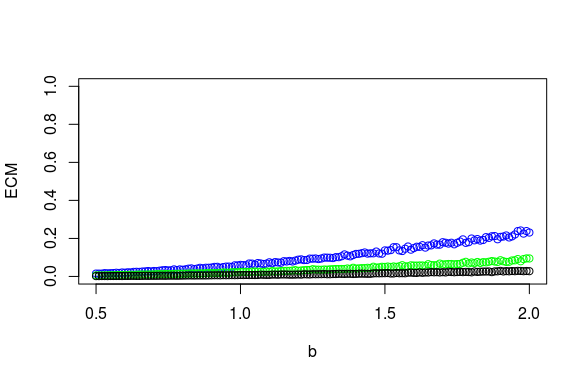
\includegraphics[scale=0.85]{ej6.png}
En este gráfico, los puntos azules representan el estimador de mediana, mientras que los verdes al de momentos y los negros al de máxima verosimilitud.
Observamos que el de máxima verosimilitud tiene menor error. Por lo tanto elegiríamos ese.

\section{Ejercicio 7}
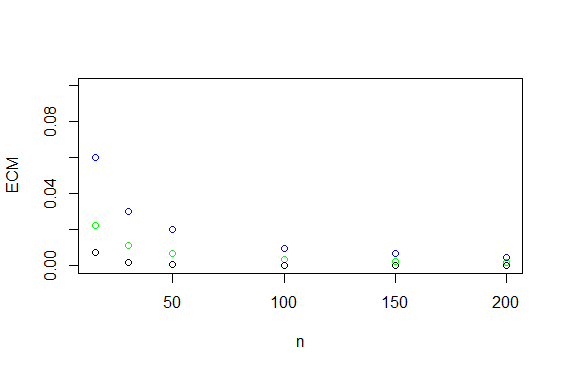
\includegraphics[scale=0.85]{ej7.png}
En este segundo gráfico, cada color representa al mismo estimador que en el Ejercicio 6.
Observamos que nuevamente el $b_{mv}$ es el que tiene menor ECM. Nos llama la atención que $b_{med}$ tenga un comportamiento tan distinto a los otros dos estimadores. Elegimos nuevamente $b_{mv}$. En todos los casos, pero particularmente en $b_{mv}$ y $b_{mom}$, observamos que el estimador se acerca al valor estimado mientras más grande es el $n$, pero se puede observar en este grafico puntualemnte, el $b_{mv}$ es el que tiene un menor ECM en los primeros 4 valores de la muestra que el $b_{mom}$. Ademas tanto el $b_{mom}$ y el $b_{mv}$ son consistentes.

\section{Ejercicio 8}
La diferencia que hay entre cada uno, al parecer el $b_{med}$ es el que se acerca mas al valor real, siendo que es uno de los valores de la muestra. Entendemos que se debe al outlayer 20.1

\newpage

\section{Ejercicio 9}
\newline

\begin{table}[h!]
\centering
\caption{Tabla comparativa}
\label{my-label}
\begin{tabular}{llll}
\hline
\multicolumn{1}{|l|}{}                  & \multicolumn{1}{l|}{\textbf{MOM}} & \multicolumn{1}{l|}{\textbf{MV}} & \multicolumn{1}{l|}{\textbf{MED}} \\ \hline
\multicolumn{1}{|l|}{\textbf{Sesgo}}    & \multicolumn{1}{l|}{0.3905915}   & \multicolumn{1}{l|}{2.823237}   & \multicolumn{1}{l|}{0.005074287}    \\ \hline
\multicolumn{1}{|l|}{\textbf{Varianza}} & \multicolumn{1}{l|}{3.441915}     & \multicolumn{1}{l|}{190.2666}    & \multicolumn{1}{l|}{0.0616792}   \\ \hline
\multicolumn{1}{|l|}{\textbf{ECM}}      & \multicolumn{1}{l|}{3.594477}     & \multicolumn{1}{l|}{198.2373}    & \multicolumn{1}{l|}{0.06170494}    \\ \hline

\end{tabular}
\end{table}
Observamos que tanto el $b_{mom}$ como el $b_{mv}$ ambos tienen un sesgo distinto a 0, mientras que el sesgo de $b_{med}$ es prácticamente 0 (es decir el valor de esperado de $b_{med}$ es b). Además, el estimador de momentos y el de máxima verosimilitud presentan varianza y ECM mucho mayor que el de $b_{med}$ (sobre todo el $b_{mv}$). Esto se debe a que el valor que está alejado del resto de los valores de la muestra (el primer elemento es cien veces más grande) hace que crezca tanto la varianza como el ECM de los primeros dos estimadores mientras que por la naturaleza del $b_{med}$ (mira el valor intermedio de la muestra), este estimador no es afectado tanto por el outlier. Elegimos el $b_{med}$ ya que no solo tiene el menor sesgo, sino también al ser resistente a valores atípicos, tiene menor ECM y varianza por lo que es más preciso y se acerca más al valor real de b.

\end{document}
